\documentclass[12pt, letterpaper]{../assignment}
\usepackage{graphicx}
\usepackage{courier}
\usepackage{minted}
\usepackage{amsmath}
\usepackage{polynom}
\usepackage{commath}
\usepackage{amssymb}
\usepackage{amsfonts} 
\usepackage{color}
\usepackage{cancel}
\usepackage{enumitem}
\usepackage{graphicx}
\usepackage{multirow}
\usepackage{float}
\usepackage{bm}
\usepackage{tikz}
\usetikzlibrary{shapes,arrows}
\usepackage{booktabs}
\usetikzlibrary{patterns}

% Define Theme Colors
\definecolor{light-gray}{rgb}{0.2,0.2,0.2}
\definecolor{header-blue}{rgb}{0,0,0.7}
% \definecolor{header-blue}{rgb}{0.5137,0.8353,0.9176}
\definecolor{header-blue}{rgb}{0,0.8,0.95}
\definecolor{dark-gray}{rgb}{0.1,0.1,0.1}
\pagecolor{dark-gray}
\color{white}

\usemintedstyle{monokai}
\oddsidemargin = 0pt
\exercisesheet{Module 6}{Assignment}
\student{Austin Barrilleaux}
\university{\color{header-blue}Johns Hopkins University}
\school{\color{header-blue}Whiting School of Engineering}
\courselabel{EN 535.612}
\semester{Fall 2024}
\usepackage[backend=bibtex,style=numeric,sorting=none]{biblatex}
\bibliography{reference}

\definecolor{light-gray}{rgb}{0.2,0.2,0.2}
\setminted{bgcolor=light-gray,frame=lines,rulecolor=white}
\setlength{\parindent}{0pt}

\makeatletter
\patchcmd{\minted@colorbg}{\noindent}{\medskip\noindent}{}{}
\apptocmd{\endminted@colorbg}{\par\medskip}{}{}
\makeatother

\begin{document}

\subsection*{EXERCISE 5.26}
\subsubsection*{Thin bar ACB is welded to a shaft that rotates at the constant angular speed $\bm{\Omega}$,
so the angle $\bm{\theta}$ between the bar and the shaft is constant.\\
(a) Derive expressions for the angular momentum $\bm{\bar{H}_C}$ and the kinetic energy of the bar.
Draw a sketch of $\bm{\bar{H}_C}$.\\
(b) Based on an analysis of the manner in which $\bm{\bar{H}_C}$ in Part (a) rotates,
derive an expression for $\bm{\frac{\partial}{\partial t}\bar{H}_C}$.\\
(c) Use Eq. (5.3.4) to evaluate $\bm{\frac{\partial}{\partial t}\bar{H}_C}$,
and compare it with the result of Part (b).}

\begin{figure}[H]
    \centering
    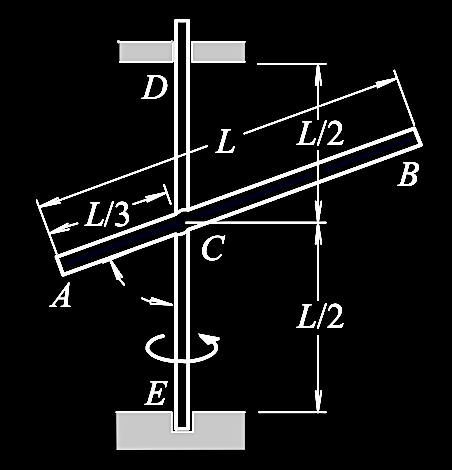
\includegraphics[scale=0.7,frame]{images/Q5_26.png}
\end{figure}

The following sketch shows the two frames of the system:

\begin{center}


    \tikzset{every picture/.style={line width=0.75pt}} %set default line width to 0.75pt        

    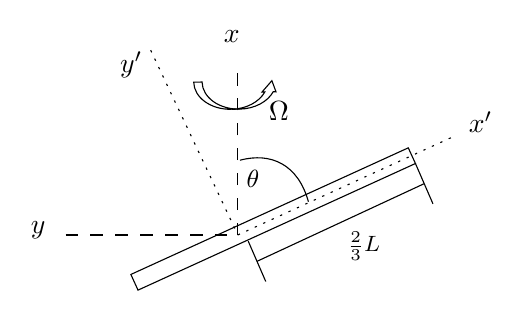
\begin{tikzpicture}[x=0.75pt,y=0.75pt,yscale=-1,xscale=1]
    %uncomment if require: \path (0,235); %set diagram left start at 0, and has height of 235
    
    %Shape: Rectangle [id:dp47104646571026665] 
    \draw   (88.45,122.03) -- (222.11,61.03) -- (225.56,68.58) -- (91.9,129.58) -- cycle ;
    %Straight Lines [id:da0462652485240338] 
    \draw  [dash pattern={on 4.5pt off 4.5pt}]  (140,103) -- (140,20) ;
    %Straight Lines [id:da2781887940807206] 
    \draw  [dash pattern={on 4.5pt off 4.5pt}]  (57,103) -- (140,103) ;
    %Straight Lines [id:da0781192111029887] 
    \draw  [dash pattern={on 0.84pt off 2.51pt}]  (140,103) -- (243,56) ;
    %Straight Lines [id:da6711962405398284] 
    \draw  [dash pattern={on 0.84pt off 2.51pt}]  (98,14) -- (140,103) ;
    %Curve Lines [id:da9209612993523657] 
    \draw    (141,67) .. controls (156,63) and (169,69) .. (174,87) ;
    %Curve Right Arrow [id:dp14539415705721326] 
    \draw  [fill={rgb, 255:red, 255; green, 255; blue, 255 }  ,fill opacity=1 ] (140.84,42.37) .. controls (130.99,42.57) and (122.9,36.72) .. (122.75,29.32) -- (118.73,29.4) .. controls (118.88,36.8) and (126.97,42.65) .. (136.82,42.45) ;\draw  [fill={rgb, 255:red, 255; green, 255; blue, 255 }  ,fill opacity=1 ] (136.82,42.45) .. controls (144.13,42.31) and (150.34,38.88) .. (153,34.09) -- (151.66,34.12) -- (156.39,28.67) -- (158.36,33.99) -- (157.02,34.02) .. controls (154.36,38.8) and (148.15,42.23) .. (140.84,42.37)(136.82,42.45) -- (140.84,42.37) ;
    %Straight Lines [id:da5955272914290781] 
    \draw    (225.56,68.58) -- (234,88) ;
    %Straight Lines [id:da5416255528259861] 
    \draw    (145,106) -- (153.44,125.42) ;
    %Straight Lines [id:da22715525047857477] 
    \draw    (149.22,115.71) -- (229.78,78.29) ;
    
    % Text Node
    \draw (143,70.4) node [anchor=north west][inner sep=0.75pt]  [font=\small]  {$\theta $};
    % Text Node
    \draw (250,42.4) node [anchor=north west][inner sep=0.75pt]    {$x'$};
    % Text Node
    \draw (132,3.4) node [anchor=north west][inner sep=0.75pt]    {$x$};
    % Text Node
    \draw (39,95.4) node [anchor=north west][inner sep=0.75pt]    {$y$};
    % Text Node
    \draw (82,13.4) node [anchor=north west][inner sep=0.75pt]    {$y'$};
    % Text Node
    \draw (153.66,37.52) node [anchor=north west][inner sep=0.75pt]    {$\Omega $};
    % Text Node
    \draw (191.5,100.4) node [anchor=north west][inner sep=0.75pt]  [font=\footnotesize]  {$\frac{2}{3} L$};
    
    
    \end{tikzpicture}
\end{center}

The rotation matrix that converts the $\{xyz\}$ frame to the $\{x'y'z'\}$ frame is:

$$ R = \left[\begin{array}{ccc} \cos\left(-\theta \right) & \sin\left(-\theta \right) & 0\\ -\sin\left(-\theta \right) & \cos\left(-\theta \right) & 0\\ 0 & 0 & 1 \end{array}\right]$$

Constructing the angular velocity vector:

$$ \bar{\omega} = \Omega\ i $$

In the body frame is:

$$ \bar{\omega} = R\ \Omega\ i =
\left[\begin{array}{r} \Omega \,\cos\left(\theta \right)\ i'\\
    \Omega \,\sin\left(\theta \right)\ j'\\
    0\ k' \end{array}\right]$$

From textbook Appendix,
the centroidal inertia mass properties of the shaft are:

\begin{equation*}
    \begin{aligned}
        I_{xx} &= 0 \\
        I_{yy} &= \frac{1}{12}m\,L^2\\
        I_{zz} &= \frac{1}{12}m\,L^2\\
    \end{aligned}
\end{equation*}

This expressed as the inertia tensor is:

$$ I_{x'y'z'} = \left[\begin{array}{ccc}
    0 & 0 & 0\\
    0 & \frac{1}{12}m\,L^2 & 0\\
    0 & 0 & \frac{1}{12}m\,L^2
\end{array}\right] $$

The distance from the body frame is:

$$ d_{x'y'z'} = \left[\begin{array}{ccc} \frac{1}{6}\,L & 0 & 0 \end{array}\right] $$

Using the parallel axis theorem to get the parallel axis transformation of inertia matrix
relative to the center of the frame of reference in question:

$$ I_{pat} = 
m\left[\begin{array}{ccc} 0 & 0 & 0\\ 0 & \frac{1}{36}\,L^2 & 0\\ 0 & 0 & \frac{1}{36}\,L^2 \end{array}\right]$$


This makes the inertia tensor at point C:

$$ I_{C} = I_{x'y'z'} + I_{pat}
m\left(\begin{array}{ccc} 0 & 0 & 0\\ 0 & \frac{1}{9}\,L^2 & 0\\ 0 & 0 & \frac{1}{9}\,L^2 \end{array}\right)$$

From this we can compute the angular momentum as:

\begin{answer}
$$ \bar{H}_C = I_{C}\ \bar{\omega} = \frac{1}{9}m\,L^2\,\Omega ,\sin\left(\theta \right)\ j' $$
\end{answer}

Since the bar rotates about the $x$ axis, the rotation component in the terminal frame that is orthogonal to the $j'$-axis is $\Omega\cos(\theta)\ i'$, therefore:
\begin{answer}
$$ \dot{\bar{H}}_C = \frac{1}{9}m\,L^2\,\Omega^2 \cos\left(\theta \right)\sin\left(\theta \right)\ k' $$
\end{answer}

If we use Eq. (5.3.4) to evaluate this, we get the same answer:

$$ \dot{\bar{H}}_C = \cancelto{0}{\frac{\partial}{\partial t} \bar{H}_C} + \bar{\omega} \times \bar{H}_C $$

\begin{answer}
\begin{equation*}
    \begin{aligned}
\dot{\bar{H}}_C &= \left[\begin{array}{r} 0 \ i'\\ 0\ j'\\ \frac{1}{9}m\,L^2\,\Omega ^2\cos\left(\theta \right)\,\sin\left(\theta \right)\ k' \end{array}\right]\\
&= \frac{1}{9}m\,L^2\,\Omega ^2\cos\left(\theta \right)\,\sin\left(\theta \right)\ k'
\end{aligned}
\end{equation*}
\end{answer}

\subsection*{EXERCISE 6.8}
\subsubsection*{The torque M acting on the gimbal of the gyroscopic turn indicator is exerted by a torsional spring, so $\bm{M = -k\beta}$.
The precession rate $\bm{\Omega_2}$ is a specified function of time,
and the spin rate $\bm{\Omega_1}$ is held constant by a servomotor.
Let $\bm{I_1}$ denote the moment of inertia of the flywheel about axis AB,
and let $\bm{I_2}$ be the centroidal moment of inertia perpendicular to axis AB.
Derive the differential equation of motion for $\bm{\beta}$.}

\begin{figure}[H]
    \centering
    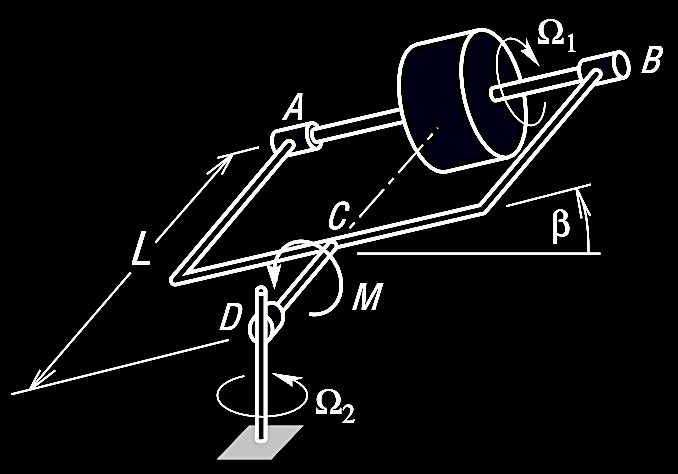
\includegraphics[scale=0.7,frame]{images/Q6_8.png}
\end{figure}


% \begin{figure}[H]
%     \centering
%     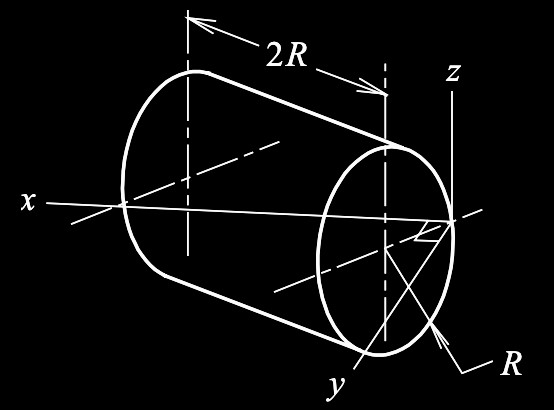
\includegraphics[scale=0.7,frame]{images/Q5_13.png}
% \end{figure}




\end{document}

